\documentclass{standalone}
\usepackage{tikz}
\usepackage{pgfplots}
\begin{document}
    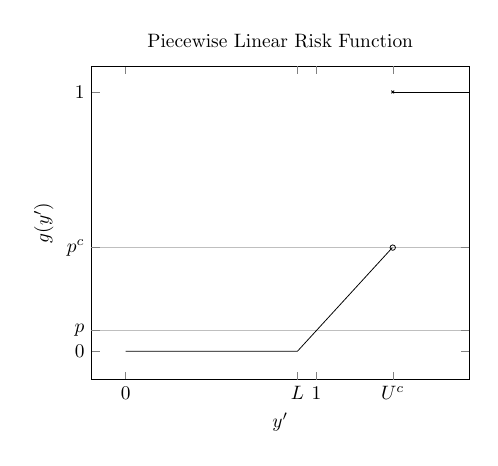
\begin{tikzpicture}[scale=.7]
      \begin{axis}[ 
	  xlabel=$y'$,
	  ylabel=$g(y')$,
	  title = Piecewise Linear Risk Function,
	  unbounded coords = jump,
	  xtick= {0},
	  ytick= {0, 1},
	  extra y ticks={.08,.4},
	  extra y tick style={grid=major},
	  extra y tick labels={$p$,$p^c$},
	  extra x ticks={.9,1,1.4},
	  extra x tick labels={$L$, 1, $U^c$},
          xmax=1.8,
          ymax=1.1,
          scatter/classes={
 	    a={mark=o,line width=3pt,scale=.75},%
 	    b={mark=o,line width=1pt,scale=1.25}%
	}]
	\addplot[black] coordinates { 
	  (0,0)		
	  (.9,0)	
	  (1.3975,.3995)		
	};	
        \addplot[black,mark=x,mark size=1pt] coordinates { (1.4,1) (2.5, 1)};
        \addplot[black,mark=o,mark size=1.4pt] coordinates{(1.4,.4)};
      \end{axis}
    \end{tikzpicture}

\end{document}
